\documentclass[12pt,a4paper]{article}
\usepackage[T1]{fontenc}
\usepackage[utf8]{inputenc}
\renewcommand{\refname}{Referências}
\renewcommand{\abstractname}{Resumo}
\renewcommand{\figurename}{Figura}
\renewcommand{\tablename}{Tabela}
\usepackage[margin=2.5cm]{geometry}
\usepackage{lmodern,microtype,graphicx,booktabs,longtable,array,amsmath,xcolor,listings,tikz}
\usepackage[hidelinks]{hyperref}
\usetikzlibrary{positioning,arrows.meta}
\definecolor{laranja}{HTML}{E85330}
\lstset{basicstyle=\ttfamily\footnotesize,breaklines=true,columns=fullflexible,frame=single,showstringspaces=false}
\setlength{\parskip}{5pt}
\setlength{\parindent}{1.2cm}
\renewcommand{\arraystretch}{1.2}
\newcommand{\pendente}[1]{\textbf{Pendente:} #1}
\title{Entre cliques: quem decide o que você vê na internet?\\\large Memorial do Projeto Final de Fundamentos de Informática}
\author{Davi Silva Vilaça\\CEFET-MG -- Campus Divinópolis\\Técnico Integrado em Informática\\Professor: Alberto Pena Lara}
\date{30 de outubro de 2026}
\begin{document}
\maketitle
\begin{center}\small
\textbf{Mídia do projeto:}\\
\url{https://quem-decide-feed-davi.jauntyharp13.chatgpt.site}\\[4pt]
\textbf{Versão de trabalho: evidências complementares pendentes.}
\end{center}
\begin{abstract}
Neste trabalho, desenvolvi o Entre cliques, um site educativo sobre como as recomendações podem mudar de acordo com nossas interações. Meu objetivo foi mostrar como curtidas e uma opção de diversidade alteram um feed fictício. O site tem um simulador, um infográfico animado e a opção de exportar resultados em CSV. Para facilitar a explicação, usei regras de pontuação que ficam disponíveis para o visitante. Neste memorial, apresento o funcionamento do produto, sua relação com os conteúdos de Fundamentos de Informática e o que ainda preciso completar. O simulador permite comparar a presença de diferentes temas, mas não reproduz todo o funcionamento de uma rede social.
\end{abstract}
\section{Introdução e caráter pessoal}
Escolhi trabalhar com a pergunta ``Quem decide o que você vê na internet?''. O que me interessou nesse tema foi entender melhor como um sistema pode selecionar os conteúdos que aparecem para uma pessoa. A partir disso, defini uma pergunta para orientar o projeto: ``Até que ponto escolho o que consumo nas redes?''.

\textbf{Meu objetivo foi criar um site educativo que mostre como curtidas e uma regra de diversidade mudam a quantidade de publicações de cada categoria em um feed fictício.}

Quis apresentar essa ideia de um jeito que outros estudantes conseguissem entender, mesmo sem conhecer programação. Por isso, escolhi uma experiência em que o visitante pode curtir conteúdos, atualizar o feed e comparar o resultado. Organizei o projeto considerando as exigências do trabalho de Fundamentos de Informática \cite{enunciado}.

\section{Descrição do problema e fundamentação}
Quando vemos uma lista de publicações, nem sempre fica claro por que aqueles conteúdos foram escolhidos. O problema que procurei abordar foi essa dificuldade de enxergar a relação entre uma interação e o que aparece depois. Para isso, escolhi um modelo pequeno, com regras que posso mostrar e explicar.

Minha ideia foi comparar duas situações: uma em que as categorias recebem espaço de acordo com os pontos acumulados e outra em que todas têm pelo menos uma vaga. Assim, é possível mudar uma regra e observar a diferença sem alterar as curtidas.

Como referência, incluí o artigo de Covington, Adams e Sargin \cite{covington}, de 2016. Ele apresenta um sistema de recomendação do YouTube com etapas de geração de candidatos e ordenação. Essa referência ajuda a perceber que os sistemas reais são mais complexos que o meu exemplo. Não usei redes neurais no simulador, nem procurei reproduzir o algoritmo atual do YouTube.

Também deixei no site uma página de suporte do TikTok como leitura complementar. Ainda preciso concluir a leitura dessa fonte antes de usar suas informações no texto. Para a parte de história dos computadores, falta aprofundar a pesquisa e relacionar a evolução dessas tecnologias com a personalização de conteúdos.

\section{Mídia produzida e funcionamento}\label{sec:modelo}
O produto que escolhi foi um site em HTML, CSS e JavaScript. Também preparei, com ajuda de IA, uma versão que pode ser aberta sem internet. O arquivo está incluído em \texttt{anexos/entre-cliques.html}. Há quatro categorias: tecnologia, música, esportes e cinema. Cada uma começa com um ponto; o feed inicial apresenta duas publicações de cada categoria.

Cada publicação pode receber uma curtida por experimento. Uma curtida acrescenta dois pontos à categoria, mas a distribuição de vagas só muda quando o visitante clica em ``Atualizar feed''. Para a categoria $i$, com $c_i$ curtidas, a pontuação é
\begin{equation}\label{eq:pontos}p_i=1+2c_i.\end{equation}
Sem a opção de diversidade, a cota ideal é
\begin{equation}\label{eq:cotas}q_i=\frac{8p_i}{\sum_{j=1}^{4}p_j}.\end{equation}
São atribuídas as partes inteiras das cotas e as vagas restantes seguem os maiores restos decimais. Em caso de empate, a ordem é tecnologia, música, esportes e cinema. Com diversidade, primeiro é atribuída uma vaga a cada categoria; as quatro vagas restantes são distribuídas proporcionalmente pelo mesmo método. A pontuação não muda ao ativar essa opção.

O programa seleciona as primeiras publicações de cada categoria até preencher a respectiva cota e intercala esses grupos. Não existe sorteio. O botão ``Reiniciar'' restaura pontos, curtidas e registros iniciais. Recarregar a página também inicia uma nova experiência.
\begin{figure}[htbp]
\centering
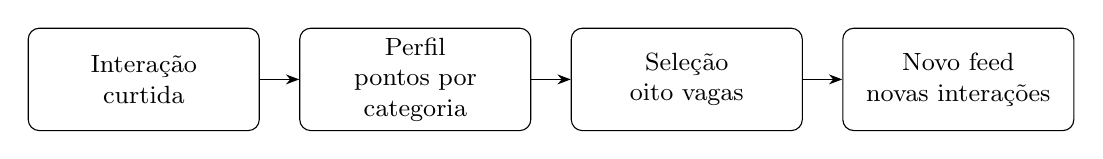
\begin{tikzpicture}[node distance=5mm, every node/.style={draw,rounded corners,align=center,text width=2.7cm,minimum height=1.3cm,font=\small},>=Stealth]
\node (a) {Interação\\curtida};
\node[right=of a] (b) {Perfil\\pontos por categoria};
\node[right=of b] (c) {Seleção\\oito vagas};
\node[right=of c] (d) {Novo feed\\novas interações};
\draw[->] (a)--(b);\draw[->] (b)--(c);\draw[->] (c)--(d);
\end{tikzpicture}
\caption{Esquema autoral do mecanismo do simulador. É uma representação explicativa, não uma captura de tela do site.}\label{fig:ciclo}
\end{figure}
A Figura~\ref{fig:ciclo} resume o mecanismo também apresentado no infográfico animado. A relação entre interação e pontuação é explícita na Equação~\ref{eq:pontos}; a relação entre pontos e vagas está na Equação~\ref{eq:cotas}.
\section{Dados, representações e condições lógicas}
\subsection{CSV e categorias}
A base de publicações é um CSV incorporado ao HTML, interpretado pelo programa e disponível para download. A cópia \texttt{anexos/publicacoes.csv} contém identificador, categoria e título. Os títulos são fictícios e educativos. A comparação exportada pelo site contém rodada, diversidade, categoria, pontos, quantidade inicial e quantidade atual. Ela não registra os identificadores individuais das curtidas; esses devem ser anotados no protocolo.
\begin{table}[htbp]\centering\small
\begin{tabular}{lll}\toprule Identificador & Categoria & Título\\\midrule
tecnologia0 & tecnologia & Por dentro de um computador\\
tecnologia1 & tecnologia & Como um pixel vira imagem\\\bottomrule
\end{tabular}
\caption{Exemplo de registros da base CSV incluída no pacote.}\label{tab:csv}
\end{table}
A Tabela~\ref{tab:csv} ilustra a organização categórica. No código, a condição de curtida verifica se o conjunto de identificadores já contém a publicação. Uma condição composta didática é: ``a publicação pertence à categoria escolhida E NÃO foi curtida''. Uma união de interesses pode ser escrita como ``tecnologia OU música''. O operador OU é aqui um exemplo de extensão possível; não se declara a existência de um filtro de duas categorias na interface atual.
\subsection{Cor, luz e bases numéricas}
Para relacionar o projeto com as bases numéricas, escolhi a cor de destaque do CSS: \texttt{\#E85330}. Em RGB de oito bits por canal, corresponde a $(232,83,48)$, como detalha a Tabela~\ref{tab:cor}. Os canais representam componentes de vermelho, verde e azul; a tripla ocupa 24 bits quando considerada sem canal alfa, metadados ou compressão.
\begin{table}[htbp]\centering
\begin{tabular}{lrrl}\toprule Canal & Hexadecimal & Decimal & Binário\\\midrule
Vermelho & E8 & 232 & \texttt{11101000}\\
Verde & 53 & 83 & \texttt{01010011}\\
Azul & 30 & 48 & \texttt{00110000}\\\bottomrule
\end{tabular}
\caption{Conversão da cor real de destaque utilizada no site.}\label{tab:cor}
\end{table}
Por exemplo, $\mathrm{E8}_{16}=14\times16+8=232$ e $232=128+64+32+8$. A cor conecta a representação de luz ao uso de bases numéricas, enquanto os rótulos textuais permitem identificar categorias sem depender apenas das cores.
\subsection{Hardware, áudio e orçamento}
\pendente{registrar processador, memória RAM, sistema operacional e navegador do computador realmente utilizado pelo aluno, explicando como afetaram o trabalho.} Não foram usadas características do ambiente de geração como se fossem as do computador pessoal.

\pendente{produzir uma narração do infográfico e anexar o arquivo, seu roteiro e propriedades reais.} O site atual não contém um arquivo de áudio. O roteiro proposto consta no Apêndice~\ref{ap:roteiro}; sua existência não comprova gravação, amostragem ou codificação de som.

\pendente{criar a planilha financeira com fórmulas e evidências.} A comparação poderá considerar hospedagem gratuita e paga, com valores, moeda, fonte e data de consulta reais. O custo anual pode ser calculado como $C_a=12C_m$ quando não houver descontos ou taxas adicionais. Não foram atribuídos preços ou gastos não pesquisados.
\section{Verificação e resultados reproduzíveis}\label{sec:testes}
Para conferir o resultado, organizei uma sequência simples: reiniciar o sistema, registrar o feed inicial, curtir uma publicação de tecnologia e atualizar. Depois, ligar a diversidade e atualizar de novo, sem adicionar curtidas. Os valores da Tabela~\ref{tab:resultados} foram conferidos pela aplicação das regras da Seção~\ref{sec:modelo}; são resultados do cálculo, não um conjunto de capturas de uma sessão do aluno.
\begin{table}[htbp]\centering\small
\begin{tabular}{lrrrr}\toprule Cenário & Tecnologia & Música & Esportes & Cinema\\\midrule
Inicial & 2 & 2 & 2 & 2\\
Uma curtida em tecnologia & 4 & 2 & 1 & 1\\
Mesma curtida, diversidade & 3 & 2 & 2 & 1\\\bottomrule
\end{tabular}
\caption{Distribuições previstas e verificáveis pelo algoritmo, sempre com oito vagas.}\label{tab:resultados}
\end{table}
Após uma curtida, os pontos são $(3,1,1,1)$. Sem diversidade, as cotas ideais são $(4,1{,}333\ldots,1{,}333\ldots,1{,}333\ldots)$: a vaga restante vai para música pelo desempate fixo. Com diversidade, as quatro vagas adicionais têm cotas $(2,0{,}666\ldots,0{,}666\ldots,0{,}666\ldots)$; a distribuição final é $(3,2,2,1)$.

A participação de tecnologia passa de 25\% para 50\% no primeiro caso e para 37,5\% com diversidade. Isso demonstra o efeito de duas regras de seleção sobre o mesmo perfil. Não demonstra comportamento de usuários reais nem mede diversidade de opiniões.

\pendente{anexar capturas dos três cenários, CSV exportado e identificação da publicação curtida; testar navegação, reinício e abertura offline.} O pacote inclui um CSV separado com os resultados calculados, identificado como tal.
\section{Matriz de articulação}\label{sec:matriz}
A Tabela~\ref{tab:matriz} contém uma linha para cada bloco do enunciado. ``Parcial'' significa que a contribuição foi iniciada, mas ainda falta evidência ou desenvolvimento. Uma atividade planejada não é apresentada como concluída.
\small
\begin{longtable}{p{.07\textwidth}p{.27\textwidth}p{.27\textwidth}p{.28\textwidth}}
\caption{Matriz de atividades, evidências e contribuições.}\label{tab:matriz}\\
\toprule Bloco & Atividade e situação & Evidência & Contribuição\\\midrule\endfirsthead
\toprule Bloco & Atividade e situação & Evidência & Contribuição\\\midrule\endhead
1A & Contextualização histórica inicial; parcial. & Introdução conceitual; pesquisa histórica específica pendente. & Situar a personalização na evolução das interfaces.\\
1B & Converter cor do site; realizado. & Tabela~\ref{tab:cor} e cálculo comentado. & Relacionar a aparência da mídia às bases numéricas.\\
1C & Documentar equipamento; pendente. & Especificações e relato ainda não anexados. & Explicar condições materiais de produção.\\
1D & Explicar RGB; realizado. & Cor real do CSS e Tabela~\ref{tab:cor}. & Mostrar representação digital de luz.\\
2A & Narrar o infográfico; pendente. & Roteiro proposto; áudio e propriedades ausentes. & Ampliar comunicação e analisar representação sonora.\\
2B & Redigir memorial em LaTeX; parcial. & Este PDF e \texttt{main.tex}. Artigo base não fornecido. & Organizar equações, tabelas e figuras em artigo.\\
2C & Citar fontes e elementos internos; realizado nesta versão. & Bibliografia, equações, figuras e tabelas referenciadas. & Tornar argumentos e registros rastreáveis.\\
2D & Descrever problema e organizar evidências; parcial. & Seção do problema e Figura~\ref{fig:ciclo}; capturas pendentes. & Explicar o propósito e permitir inspeção do produto.\\
3A & Comparar custos; pendente. & Planilha financeira ainda ausente. & Justificar escolha de hospedagem com cálculos.\\
3B & Categorizar e compor condições; parcial. & Base e condições descritas; OU apresentado como extensão. & Explicar classificação e decisões de seleção.\\
3C & Usar e exportar CSV; realizado no produto. & Base anexa e rotina de exportação; sessão documentada pendente. & Permitir reutilizar dados e comparar rodadas.\\
3D & Produzir infográfico; realizado no site. & Seção do ciclo no HTML e esquema da Figura~\ref{fig:ciclo}. & Comunicar o funcionamento para iniciantes.\\
3E & Organizar planejamento; parcial. & Links do mapa e Trello, cofre Obsidian e snippet. Capturas pendentes. & Registrar etapas, decisões e reaproveitamento de código.\\
\bottomrule
\end{longtable}\normalsize
\section{Planejamento e evidências existentes}
Para organizar o projeto, usei um mapa mental no Xmind, um quadro no Trello e notas no Obsidian. A IA me ajudou a montar essa estrutura. Esses materiais reúnem as decisões e tarefas do projeto, mas não são um registro automático de tudo o que fiz antes de criá-los.
\begin{itemize}
\item Mapa mental: \url{https://app.xmind.com/share/MGqWHt1g}.
\item Trello: \href{https://trello.com/b/fPSRjyWN/entre-cliques-projeto-final-de-fui}{Quadro do projeto no Trello}.
\item Obsidian: notas Markdown incluídas na pasta \texttt{obsidian} deste pacote.
\end{itemize}
O mapa apresenta objetivo, mecanismo, produto, verificação, conteúdos e planejamento. O quadro possui listas de orientação, tarefas a fazer, em andamento, em revisão e concluídas. As notas do Obsidian distinguem material existente de pesquisa e evidências pendentes. Um trecho reutilizável do programa está no Apêndice~\ref{ap:codigo}. As capturas dessas ferramentas e os registros das próximas alterações devem ser inseridos em uma revisão do memorial.
\section{Uso de inteligência artificial}
Usei o ChatGPT para criar e hospedar o site, incluindo ajuda com a programação, o visual e o simulador. Também usei a IA para organizar o projeto: estruturar o mapa mental, montar as tarefas do Trello e preparar as notas do Obsidian.

Na elaboração deste memorial, a IA ajudou na redação, na revisão e na formatação em LaTeX. Esse apoio não substitui minha responsabilidade de conferir o conteúdo e entender o funcionamento do que estou apresentando. As atividades que ainda não têm evidências estão identificadas no texto, para que eu possa completá-las antes da entrega.

\section{Considerações finais}
Com o Entre cliques, consegui transformar uma pergunta ampla em um exemplo que pode ser observado e explicado. A comparação mostra que o mesmo perfil de pontos pode gerar feeds diferentes quando a regra de seleção muda.

O principal resultado é a possibilidade de acompanhar essa mudança e entender de onde ela veio. Ao mesmo tempo, preciso respeitar o limite do exemplo: ele trata da quantidade de temas em um feed fictício e não permite tirar conclusões sobre o comportamento de todas as redes sociais.

Ainda preciso completar os itens indicados na matriz, principalmente as informações do computador, o áudio, a planilha e as capturas. Também falta adaptar o memorial ao artigo base do professor, quando ele estiver disponível. Antes da entrega, vou precisar revisar esses registros e conferir o acesso ao site.

\begin{thebibliography}{9}
\bibitem{enunciado} LARA, Alberto Pena. \textit{Fundamentos de informática: trabalho individual}. CEFET-MG, Campus Divinópolis, 2026. Enunciado disponibilizado nas fontes do projeto, 4 p.
\bibitem{covington} COVINGTON, Paul; ADAMS, Jay; SARGIN, Emre. \textit{Deep Neural Networks for YouTube Recommendations}. Proceedings of the 10th ACM Conference on Recommender Systems, 2016. Página institucional: \url{https://research.google/pubs/deep-neural-networks-for-youtube-recommendations/}. Consulta nesta etapa: 30 out. 2026.
\end{thebibliography}
\appendix
\section{Roteiro proposto para narração}\label{ap:roteiro}
``Quando você curte uma publicação neste simulador, a categoria ganha dois pontos. Ao atualizar, o programa distribui oito vagas de acordo com esses pontos. Uma categoria que recebe mais curtidas pode ganhar mais espaço. Ao ligar a opção de diversidade, cada categoria recebe pelo menos uma vaga. Compare os resultados com as mesmas curtidas. Esta experiência usa regras programadas: ela ajuda a entender a seleção, mas não reproduz todas as decisões de uma rede social.''

Este é um roteiro proposto, ainda sem gravação anexada.
\section{Snippet da distribuição}\label{ap:codigo}
A função abaixo corresponde à lógica do HTML disponível. Os nomes foram preservados e a apresentação foi dividida em linhas para facilitar a leitura.
\begin{lstlisting}
function allocate(weights, diverse) {
  const base = diverse ? 1 : 0;
  const total = weights.reduce((a,b) => a+b, 0);
  const ideals = weights.map(w => w/total*(8-base*4));
  const n = ideals.map(x => Math.floor(x)+base);
  const order = ideals.map((x,i) =>
    ({i, r:x-Math.floor(x)}))
    .sort((a,b) => b.r-a.r || a.i-b.i);
  let remaining = 8-n.reduce((a,b) => a+b, 0);
  for(let j=0; j<remaining; j++) n[order[j].i]++;
  return n;
}
\end{lstlisting}
\end{document}
